\documentclass[11pt,a4paper]{article}
\usepackage[margin=27mm]{geometry}
\usepackage{fontspec,booktabs,array,hyperref,graphicx}
\setmainfont{STIXGeneral}
\setlength{\parindent}{0pt}\setlength{\parskip}{5pt}
\begin{document}
\begin{center}{\Large Complete manuscript comparison}\\[3pt]
Overview v14: unified A and three-source Mixes\end{center}
There are 18 topics and 47 recovered originals among 106 accessible originals; 59 remain pending and 55 earlier indexed originals remain archived. A combines the eight originals previously assigned to A and Affine. Mixes now includes F007 alongside F005 and L016. The other 16 topic records and 36 individual records retain their exact v13 boundaries, including expanded E and the symmetric listing corrections.

For each topic the complete written factor is $\sum_i c(S_i)/(c(U)+\sum_i c(A_i))$. Whole common theory and all complete applications are paid once within that topic. Each row retains its independently adopted nonwhitespace-character coordinate; there is no cross-topic discount, pooled factor or inferred minimum proof complexity. Concrete software listings are excluded on both sides. Proof and mathematical algorithm prose remain counted.
\begin{center}\small\begin{tabular}{lrrrrr}\toprule
Topic & Originals & Sources & Common & Applications & Factor\\\midrule
A & 8 & 246,570 & 66,140 & 110,576 & 1.395 \\
B & 5 & 124,906 & 44,905 & 69,265 & 1.094 \\
C & 5 & 118,433 & 30,437 & 61,248 & 1.292 \\
D & 3 & 47,894 & 15,632 & 29,855 & 1.053 \\
E & 5 & 140,286 & 57,473 & 32,337 & 1.562 \\
F & 2 & 69,825 & 15,876 & 27,398 & 1.614 \\
G & 2 & 73,199 & 30,928 & 85,207 & 0.630 \\
Representation & 1 & 25,348 & 11,288 & 13,688 & 1.015 \\
Chamber & 2 & 34,177 & 15,199 & 21,254 & 0.938 \\
Matching & 1 & 37,951 & 16,732 & 17,168 & 1.119 \\
ChiralEnumeration & 1 & 27,594 & 8,831 & 23,171 & 0.862 \\
Operations & 3 & 200,630 & 58,215 & 100,379 & 1.265 \\
Gluing & 1 & 27,081 & 28,416 & 11,565 & 0.677 \\
RankContraction & 1 & 15,530 & 6,937 & 10,555 & 0.888 \\
LocallyProjective & 2 & 26,490 & 25,498 & 11,966 & 0.707 \\
MathieuCensus & 1 & 13,736 & 5,516 & 35,862 & 0.332 \\
RankAugmentation & 1 & 33,604 & 13,904 & 14,096 & 1.200 \\
Mixes & 3 & 156,570 & 34,757 & 68,693 & 1.513 \\
\bottomrule\end{tabular}\end{center}
The \href{topics.csv}{18-topic CSV} and \href{applications.csv}{47-original CSV} preserve exact fractions, complete component lengths and historical observations. Factors below one remain visible. The source maps and separate admissions determine the recovered principal contracts; this numerical overview adds no separate proof or question credit.
\newpage
\section*{Individual comparisons: first 24 originals}
After acquiring the \emph{whole} common theory and all actual required mathematical, computational and data premises, the conditional factor is $c(S_i)/c(A_i)$. The complete local application or companion bundle remains charged.
\begin{center}\small\begin{tabular}{llrrr}\toprule
Original & Topic & Source & Application & Factor\\\midrule
L032 & A & 16,558 & 8,228 & 2.012 \\
L034 & A & 21,433 & 5,801 & 3.695 \\
F016 & A & 43,983 & 15,436 & 2.849 \\
F013 & A & 25,562 & 6,241 & 4.096 \\
L035 & A & 51,019 & 14,514 & 3.515 \\
N009 & A & 36,824 & 28,130 & 1.309 \\
L128 & A & 18,424 & 8,825 & 2.088 \\
L012 & A & 32,767 & 23,401 & 1.400 \\
N001 & B & 14,519 & 7,371 & 1.970 \\
N003 & B & 17,780 & 9,155 & 1.942 \\
N008 & B & 18,009 & 11,132 & 1.618 \\
L030 & B & 22,704 & 12,286 & 1.848 \\
L040 & B & 51,894 & 29,321 & 1.770 \\
L088 & C & 13,166 & 11,311 & 1.164 \\
N013 & C & 27,361 & 15,815 & 1.730 \\
L108 & C & 12,849 & 10,075 & 1.275 \\
F014 & C & 20,577 & 6,962 & 2.956 \\
L068 & C & 44,480 & 17,085 & 2.603 \\
L066 & D & 20,916 & 10,989 & 1.903 \\
L074 & D & 20,661 & 13,367 & 1.546 \\
L104 & D & 6,317 & 5,499 & 1.149 \\
L079 & E & 21,212 & 1,858 & 11.417 \\
L083 & E & 20,904 & 2,922 & 7.154 \\
L021 & E & 29,594 & 14,452 & 2.048 \\\bottomrule\end{tabular}\end{center}
Unified A pays its full 23-page common paper and all 45 application pages. Its source total is 246,570 characters and its replacement is $66,140+110,576=176,716$, giving $123285/88358$. The primary coordinate remains calibrated selected extraction, NFC, without whitespace. Neither earlier A theory nor earlier Affine theory is free. Graphical structure and unextracted image labels remain unknown costs.

All eleven required program/data files remain required even though software is outside this manuscript factor. Three inherited auxiliary files, two current drivers and fourteen partial formal files remain separately inventoried. Their whole-file costs are preserved; no full-formalization claim or software-inclusive factor follows.
\newpage
\section*{Individual comparisons: remaining 23 originals}
\begin{center}\small\begin{tabular}{llrrr}\toprule
Original & Topic & Source & Application & Factor\\\midrule
L056 & E & 15,871 & 4,144 & 3.830 \\
L043 & E & 52,705 & 8,961 & 5.882 \\
L014 & F & 25,574 & 11,504 & 2.223 \\
L007 & F & 44,251 & 15,894 & 2.784 \\
L009 & G & 49,891 & 23,544 & 2.119 \\
L092 & G & 23,308 & 61,663 & 0.378 \\
F010 & Representation & 25,348 & 13,688 & 1.852 \\
L008 & Chamber & 20,159 & 7,571 & 2.663 \\
N016 & Chamber & 14,018 & 13,683 & 1.024 \\
F015 & Matching & 37,951 & 17,168 & 2.211 \\
L028 & ChiralEnumeration & 27,594 & 23,171 & 1.191 \\
N005 & Operations & 122,002 & 49,595 & 2.460 \\
N006 & Operations & 55,740 & 38,479 & 1.449 \\
N007 & Operations & 22,888 & 12,305 & 1.860 \\
L010 & Gluing & 27,081 & 11,565 & 2.342 \\
L037 & RankContraction & 15,530 & 10,555 & 1.471 \\
L084 & LocallyProjective & 2,071 & 4,857 & 0.426 \\
L095 & LocallyProjective & 24,419 & 7,109 & 3.435 \\
L073 & MathieuCensus & 13,736 & 35,862 & 0.383 \\
L020 & RankAugmentation & 33,604 & 14,096 & 2.384 \\
F005 & Mixes & 57,753 & 31,077 & 1.858 \\
L016 & Mixes & 35,506 & 15,125 & 2.348 \\
F007 & Mixes & 63,311 & 22,491 & 2.815 \\\bottomrule\end{tabular}\end{center}
Mixes pays three common papers: $12,615+11,641+10,501=34,757$. The complete applications cost 31,077 for F005, 15,125 for L016 and 22,491 for F007. Thus its full comparison is $156570/(34757+68693)=15657/10345$. Its primary is raw untrimmed extraction, NFC, without whitespace. Both required finite certificates remain required; the REQ appendix prints both files. Six validation programs remain optional; six drivers and three partial formal files are separately inventoried.

F005's three final problems remain unanswered. L016 retains the faithful repair of its thin-cover lemma and its ancillary exclusions. F007's page-25 chain-class paragraph is not recovered; Problems 1 and 2 remain unanswered. Its Problem 3 result has the stated natural-reconstruction and finite connected-flag-graph scope, with no general infinite or priority claim. Twelve partial Lean declarations are not full source formalization.

Historical software, retained external proofs, complete graphics and full formalization costs remain unknown. All software-inclusive and pooled factors are null. Operations retains its separate text-only sensitivity; expanded E retains its accepted source qualifications and the source's Magma/$L_2$-quotient attribution. Prior overviews remain historical records.
\newpage
\section*{Whole topics}
Grey bars show the complete original manuscript text in each row's adopted coordinate. Replacement bars stack the entire common theory and all applications. The axis starts at zero; the tables give the ratios.
\begin{center}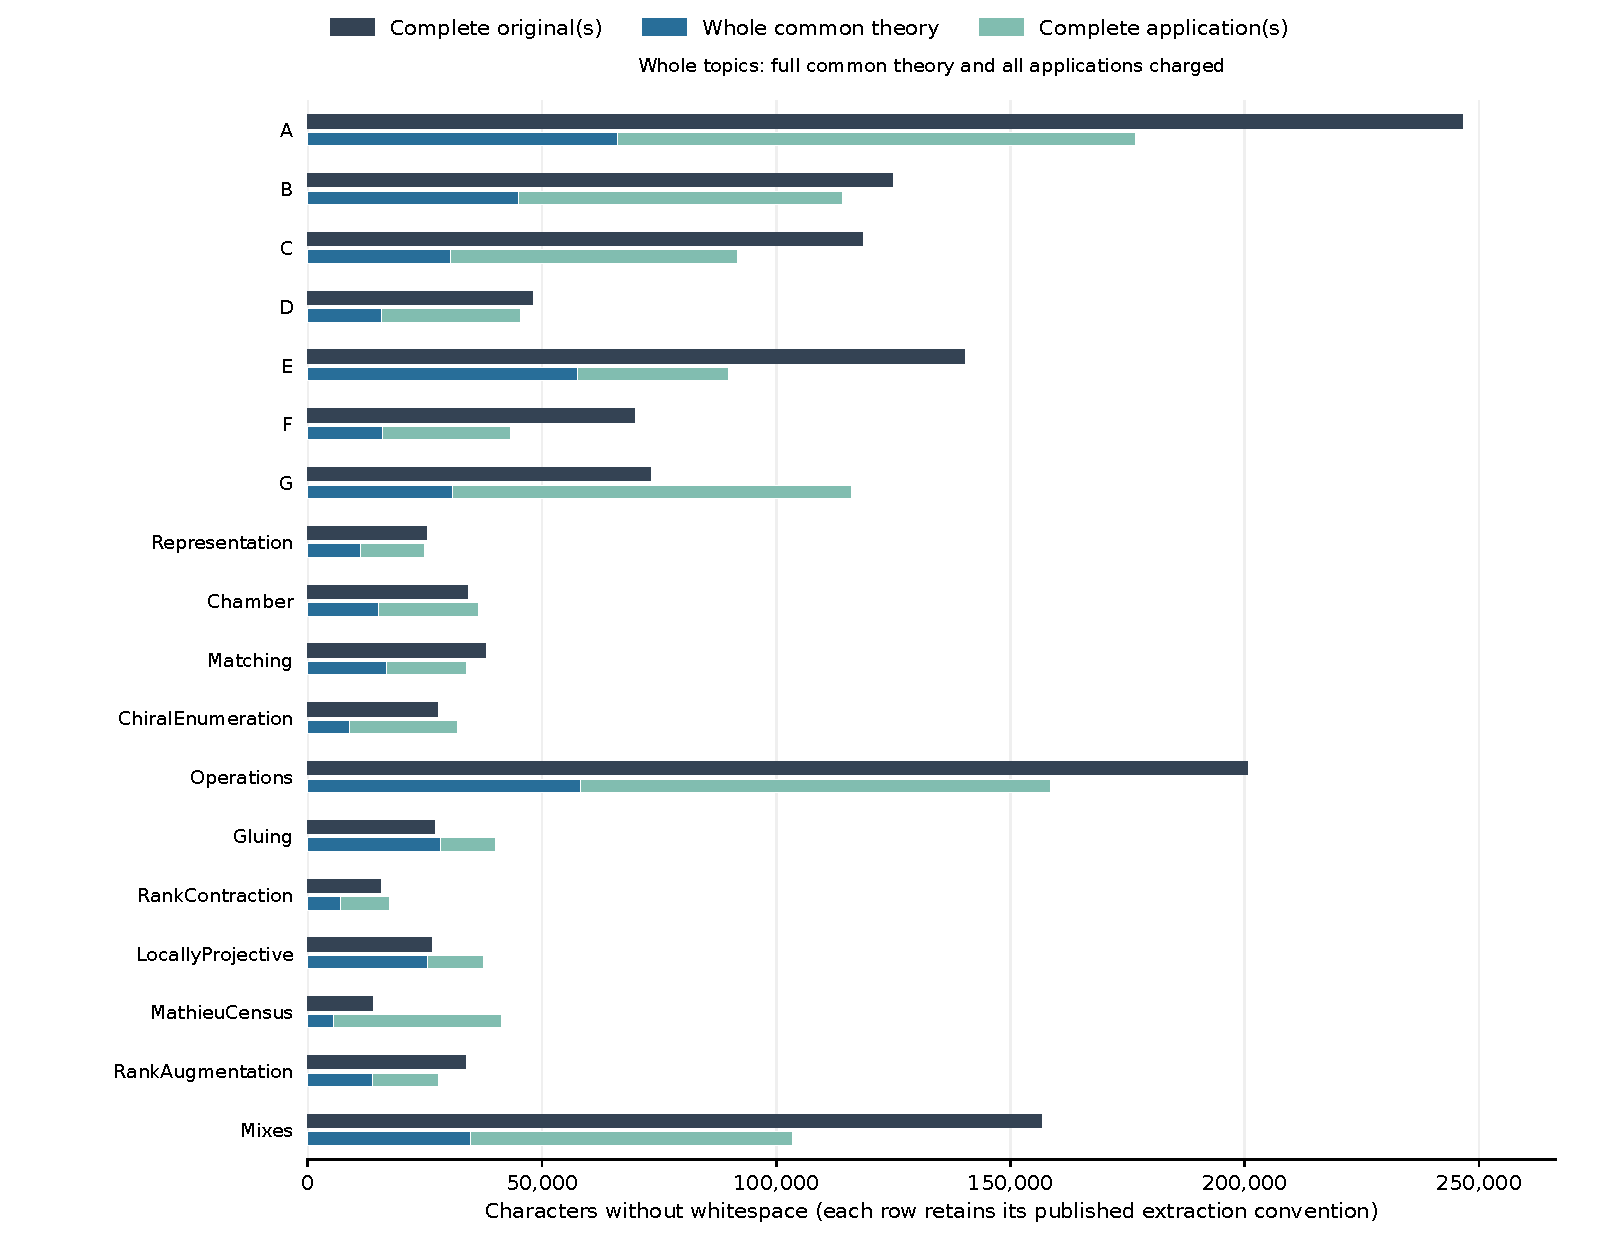
\includegraphics[width=\linewidth]{whole_topics.pdf}\end{center}
The 54 bars account for all 18 topics. No necessary finite certificate or external premise becomes optional merely because software and retained external proof costs are outside the manuscript coordinate.
\newpage
\section*{Conditional lengths: first 24 originals}
Whole common theory and required premises are acquired in advance. Grey and teal bars compare complete source and local application text; the whole-topic table still pays the common theory.
\begin{center}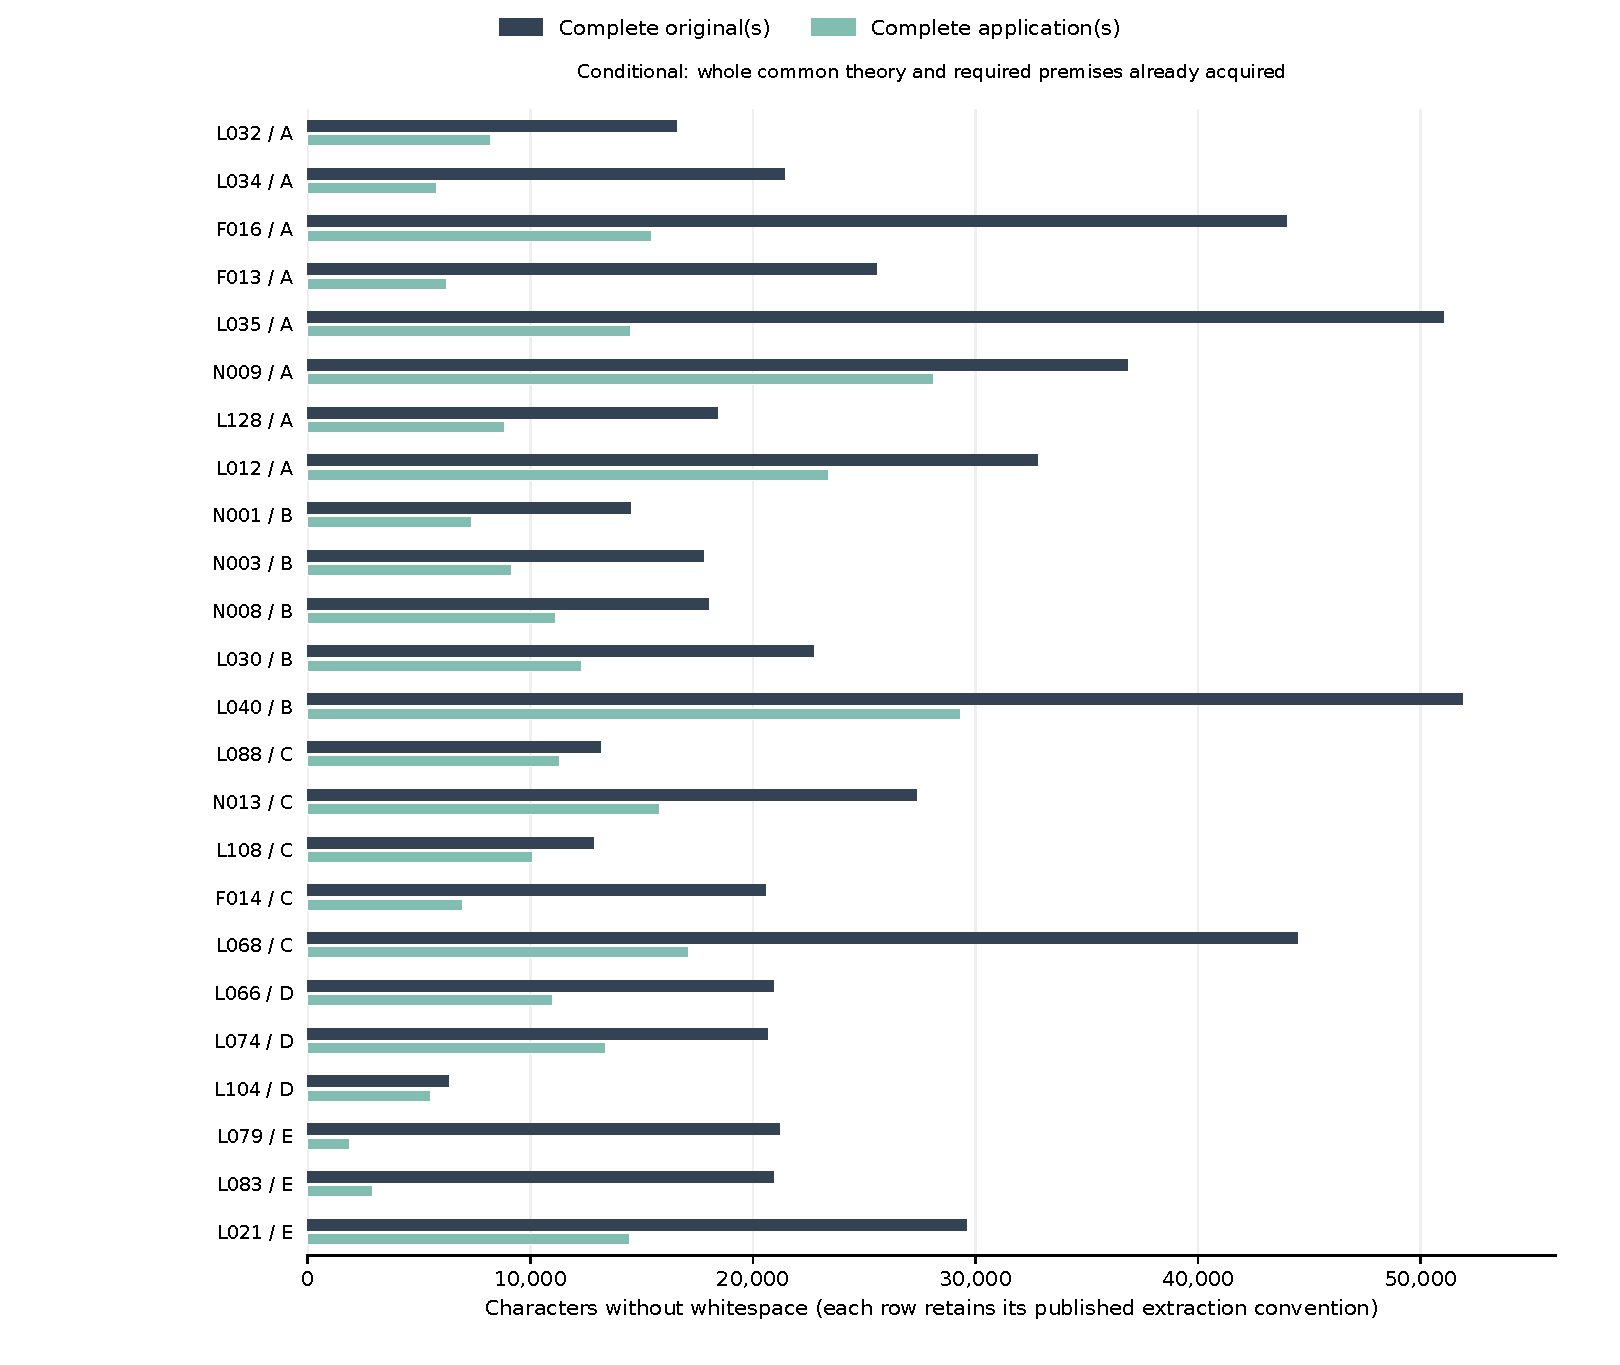
\includegraphics[width=\linewidth]{conditional_1.pdf}\end{center}
\newpage
\section*{Conditional lengths: remaining 23 originals}
All complete companion papers remain charged. The source order is documentary, not an optimal acquisition order or a claimed sawtooth.
\begin{center}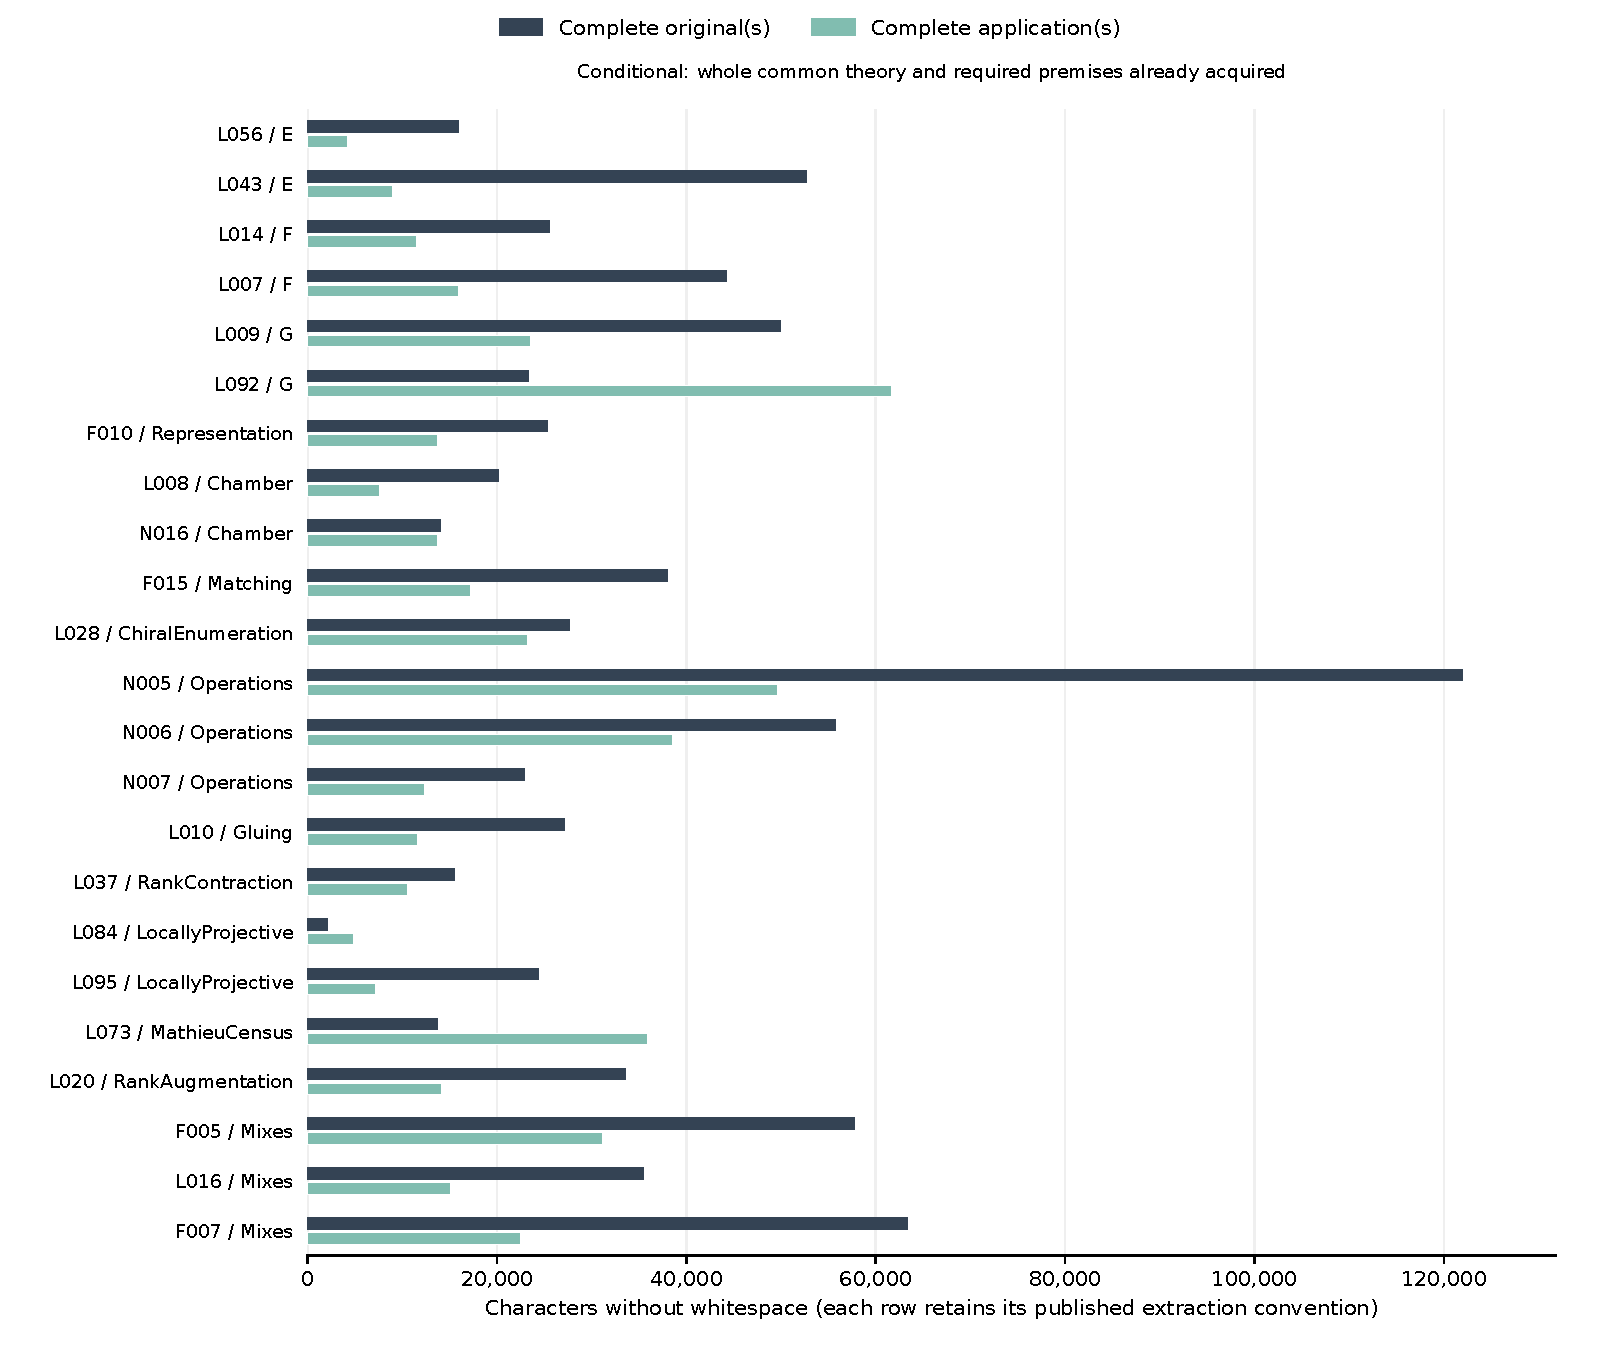
\includegraphics[width=\linewidth]{conditional_2.pdf}\end{center}
This edition supplies 65 exact written comparisons and 148 plotted bars. The active programme remains 106 originals, with 47 recovered and 59 pending. Only F007 is newly reflected from its separate scientific admission; the A--Affine merger changes topic organization, not the number of originals.
\end{document}
